\noindent1.The one-time capture feature on an oscilloscope allows you to capture and display a single, non-repetitive event or waveform.\\ 2.Unlike regular oscilloscope operation, which continuously displays repeating signals, the one-time capture freezes the oscilloscope's display after it detects a specific event, such as a glitch or an unexpected signal, that occurs only once or very infrequently.\\3. This is especially useful for analyzing rare issues that may not happen again during testing.
4.In this mode, the oscilloscope uses its trigger settings to capture the exact moment the event occurs.\\5. Once triggered, the oscilloscope captures the waveform and stores it in its memory for further analysis.\\ 6.This feature helps engineers diagnose problems that are hard to reproduce, making it easier to investigate and troubleshoot transient or irregular signals.
\subsection{Steps in one time capture}
\begin{itemize}
    \item Set the mode of oscilloscope to \textbf{Burst} mode.
    \item Select the trigger option in Function Generator.
    \item Set the number of bursts i.e, Number of Cycles to be captured.
    \item Connect the probes.
    \item The Number of cycles we have selected will be displayed on the screen .
\end{itemize}
\subsection{Example of One-time capture}
Here is the example of One-time capture of a square wave in which we took 7 Cycles ,\\
 \begin{figure}[h!]
    \centering
    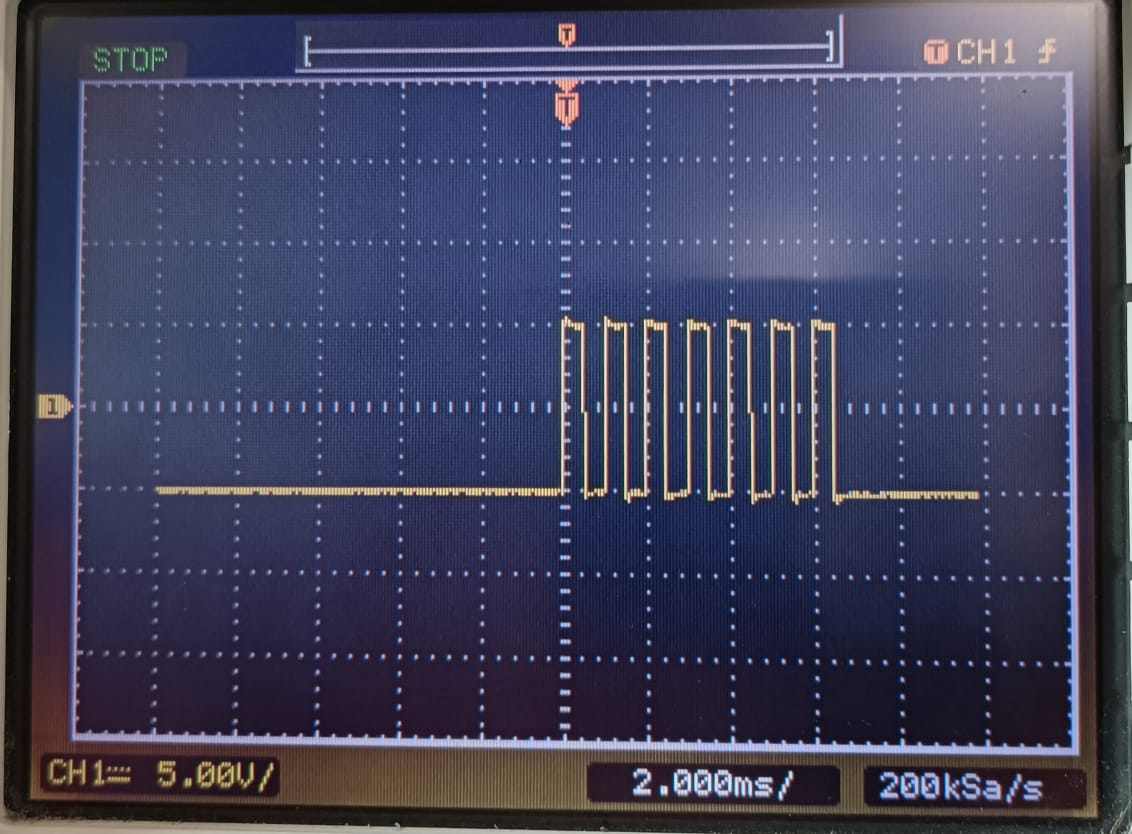
\includegraphics[width=0.45\textwidth]{actualgraph/7cycles.jpeg}
    \caption{Graph of above signal using python}
    \label{fig:sample_image}
     \end{figure}
     \newpage
Here is the picture of function generator related to above picture, \\
\begin{figure}[h!]
    \centering
    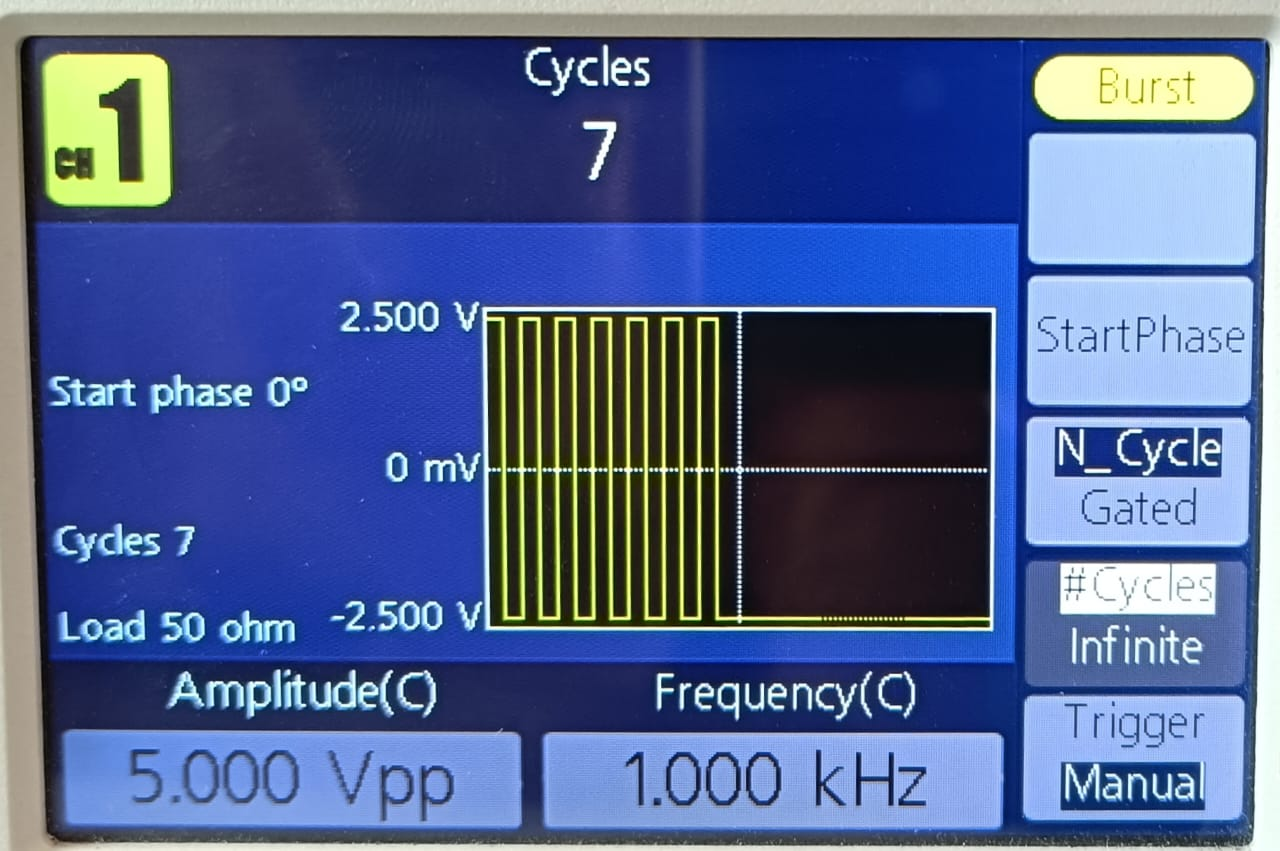
\includegraphics[width=0.6\textwidth]{actualgraph/funcgen.jpeg}
    \caption{Graph of above signal using python}
    \label{fig:sample_image}
     \end{figure}
